% !TeX encoding = UTF-8
% !TeX spellcheck = en_GB
\documentclass[a4paper]{article}

\usepackage[utf8]{inputenc}
\usepackage[T1]{fontenc}
\usepackage{lipsum}
\usepackage{enumitem,kantlipsum}
\usepackage{verbatim}
\usepackage{graphicx}

\graphicspath{ {images/} }

\title{Pollution Detection System\\User Manual}
\author{PLA25}

\begin{document}

\maketitle
\vspace*{\fill}

\paragraph{Group members}
\begin{tabbing}
	Joey Blankendaal 	\` 	500778751 	\\
	Thom de Jong 		\` 	500778147 	\\
	Brian Karmelk 		\` 	500768939 	\\
	Matthijs Snijders 	\` 	500780453 	\\
	Martijn Vegter 		\` 	500775388
\end{tabbing}

\thispagestyle{empty}
\newpage

\tableofcontents
\newpage

\section{Introduction}

\subsection{Who are we?}
We are a group of students who go by the name of PLA25. We are currently studying at the Amsterdam University of Applied Sciences. Our group consists of software engineering and technical computing students.

\subsection{Our product}
The Pollution Detection System (PDS) is a web-based application that provides information about the pollution on earth. Both light pollution and air pollution are being monitored using this system.
\newline
\newline
The system uses so called "sensorhubs". Sensorhubs are a combination of multiple sensors inside of a box. These sensorhubs can be placed in a specific area to measure the pollution. These measurements can be monitored using the PDS website. This can be done by using the website's main feature, the map.
\newline
\newline
The system uses sensors that can be placed in a specific area to measure the pollution. These measurements can be monitored using the PDS website. This can be done by using the website's main feature, the map.

\newpage
\section{The website}
\subsection{The login and logout.}
The login page is simple, use your username and password to login to the website. The website uses a role system, which means there are two roles a user of the website can be. You're either an admin or a user. 

\begin{enumerate}[]
	\item Use the upper input field for your username.
	\item Use the lower one for your password.
	\item Finally, click the "login" button.
\end{enumerate}
\noindent
After completing these steps you are being redirected to the homepage.
\newline
\newline
On the top of this website there is a navigation bar, which is used to visit the several available pages. These pages include: the home page the map page and the admin page. The latter is only shown if the current user is an admin.
\newline
\newline
If you want to log out, simply click the logout button at the very end of the navigation bar (see figure 2).
\newline
\newline
The login page contains buttons to switch between the languages Dutch and English (see figure 1).
\newline
All other pages also have these buttons in their dropdown menu(see figure 2).
\newline


\begin{figure}[h!]
  \caption{The login page.}
  \centering
  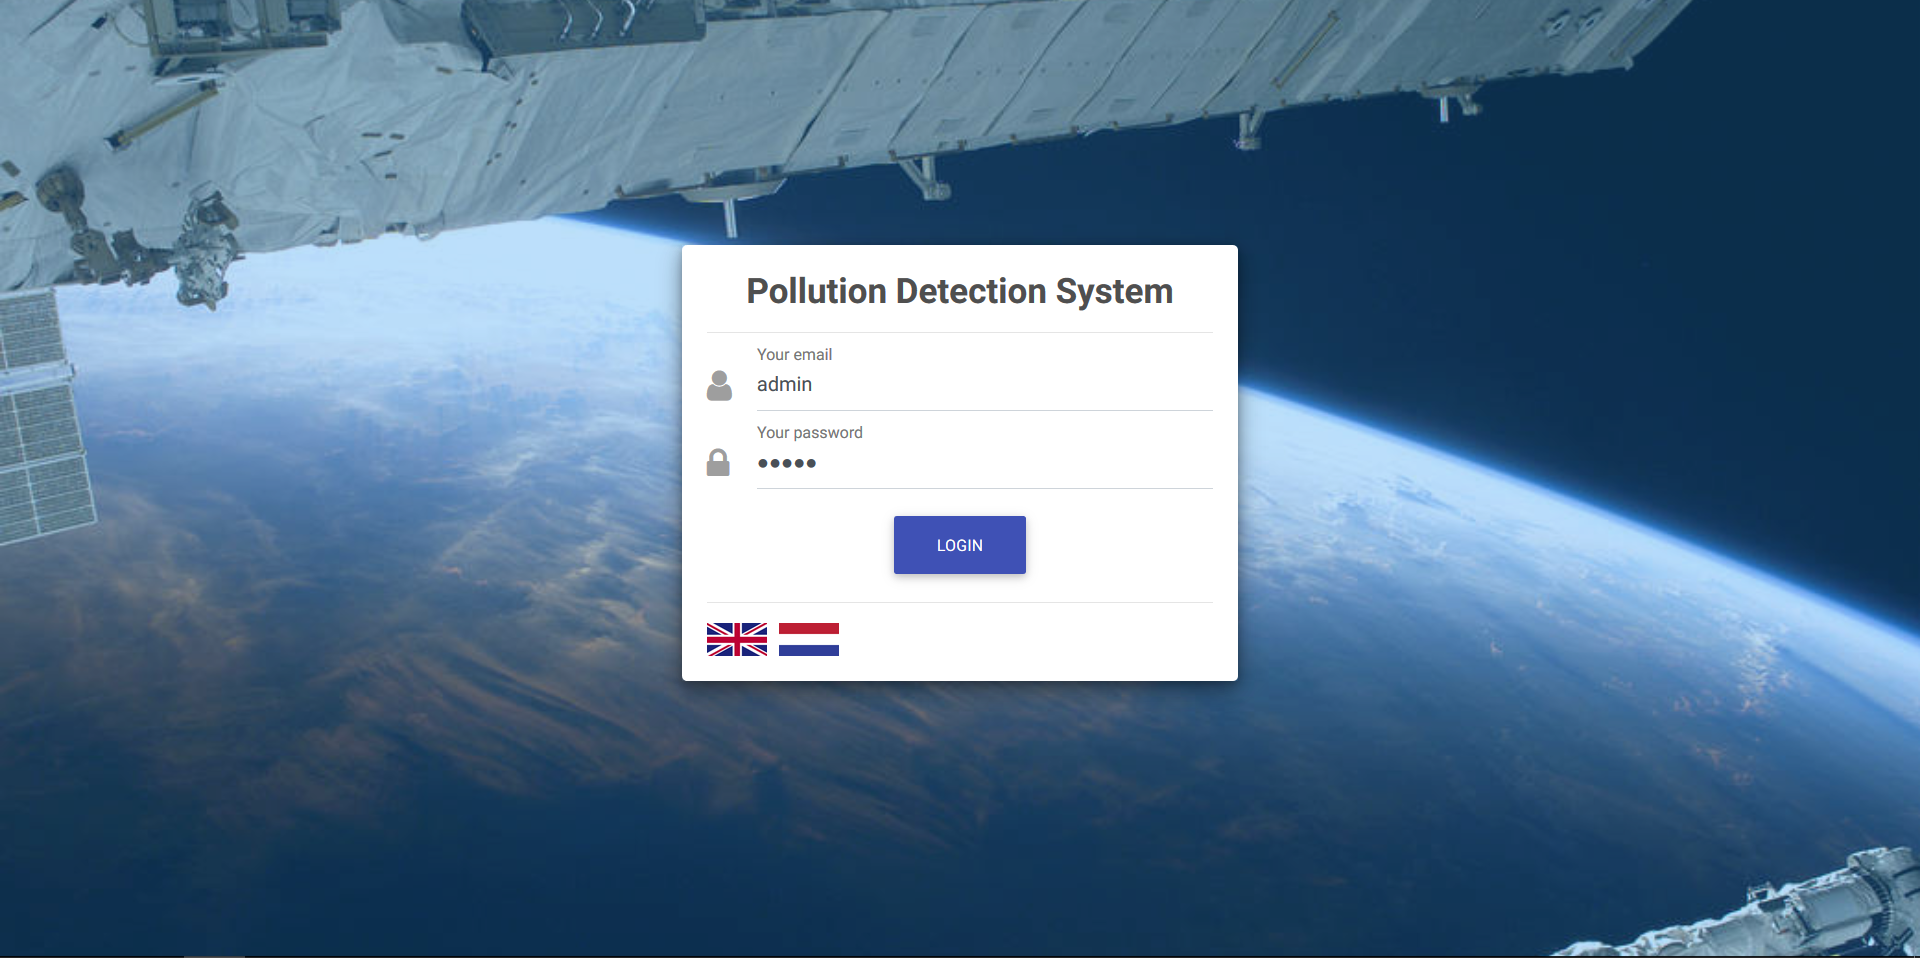
\includegraphics[width=1\textwidth]{login}
\end{figure}

\pagebreak

\subsection{The homepage.}
Once the user has logged in to the website the user will be redirected to the home page of our website. On the home page the user will see a navigation bar at the top of the web page. On the navigation bar there will be several buttons. These buttons vary per user depending if the user is a admin or a user. 
\newline
\newline
On the home page itself the user will see a short welcome message as well. In the welcome message we introduce the user to our website and explain the features we have on our website. The home page also contains links to our blog, GitHub and more information for help.
\begin{figure}[h!]
  \caption{The homepage with an opened dropdown menu.}
  \centering
  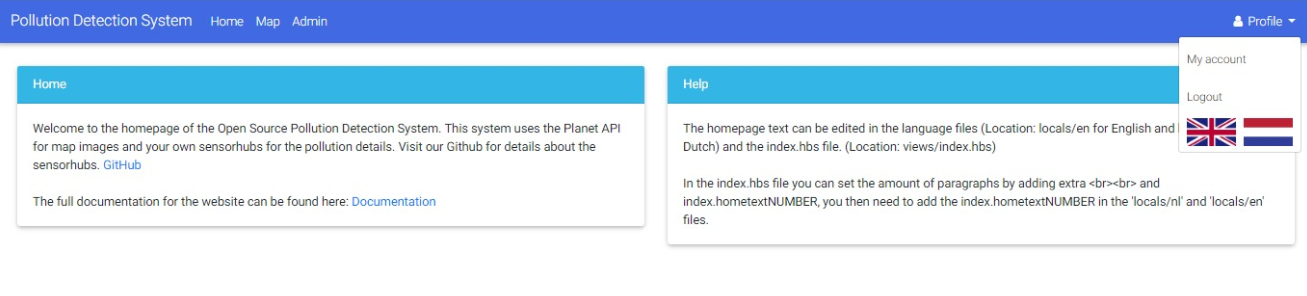
\includegraphics[width=1\textwidth]{home-dropdown}
\end{figure}
\pagebreak

\subsection{The map page}
This page is the primary feature of our product; the map. This map consists of data gathered by our sensor hubs. On the left you can see a smaller box called "Options", where you can filter out certain types data and view details about them. On the right you can see a larger called "Map", which is our interactive map that derives its display from what is selected in the Options menu.
\newline

\subsubsection*{Searching for a specific location}
Want to find out the pollution of a specific location? See figure 2 and follow these steps:
\begin{enumerate}
\item Click on the search bar in the Options menu.
\item Type in your desired location.
\item (optional) Click on a suggestion that meets your criteria.
\item (optional) Zoom in or out.
\end{enumerate}
\begin{figure}[h!]
  \caption{Search bar.}
  \centering
  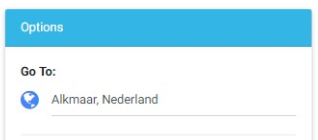
\includegraphics[width=0.5\textwidth]{search}
\end{figure}
The search bar can also search with coordinates instead of names. It's not possible to search outside of the Netherlands.
\newline

\subsubsection*{Filtering out map layers}
Do you think there's too much information on the map? It's possible to filter specific layers out. See the figure below and follow these steps:
\begin{enumerate}
\item Go to the Features and Layers part of the Options menu.
\item Click on Navigation if you want to show/hide the roads on the map.
\item Click on SensorHubs if you want to show/hide the sensor hubs on the map.
\item Click on Temperature if you want to show/hide the temperature data on the map.
\item Click on Gasses if you want to show/hide the gas pollution data on the map.
\item Click on Light if you want to show/hide the light pollution data on the map.
\end{enumerate}
\begin{figure}[h!]
  \caption{Features and layers.}
  \centering
  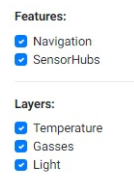
\includegraphics[width=0.3\textwidth]{features-layers}
\end{figure}
These layers are stacked on top of each other. The Planet API layer is the base layer that's always present. The features and layers in the Options menu are all displayed or hidden based on the user's choice. This gives you the maximum amount of choice over how you want to view our data.
\newline

\subsubsection*{Viewing data from the past}
Want to find out about data from the past? See the figure below and follow these steps:
\begin{enumerate}
\item Go to the Timeline part of the Options menu.
\item (option 1) Click on the selector and select how far you want to go back.
\item (option 2) Drag the timeline bar to how far you wish to go back.
\end{enumerate}
\begin{figure}[h!]
  \caption{Timeline.}
  \centering
  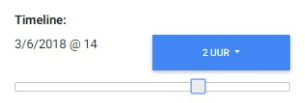
\includegraphics[width=0.6\textwidth]{timeline}
\end{figure}
As you can see, the Timeline part also displays the current selected date and time. The format is MM/DD/YYYY @ HH. Since we don't save data more often than once an hour, there's only the hour number displayed.

\newpage
\subsubsection*{Help with reading the map data}
Don't know what the displayed data on the map means? See the figure below and follow these steps:
\begin{enumerate}
\item Click on the Map Information button in the Options menu.
\item Pinpoint the type of pollution you want to know about and read the instructions.
\end{enumerate}
\begin{figure}[h!]
  \caption{Map information.}
  \centering
  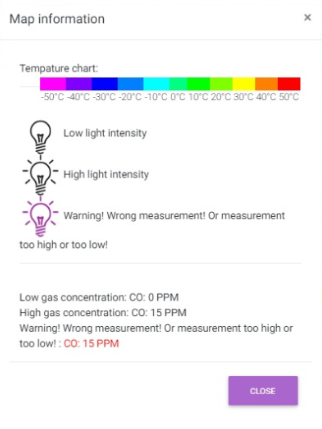
\includegraphics[width=0.7\textwidth]{legend}
\end{figure}
The map information also covers abnormal measurements of data, in case that occurs.

\newpage
\subsubsection*{Viewing the averages of the last 24 hours of a sensor hub location}
By following the steps and the figure below, you are able to see the averages  of the last 24 hours of a sensor hub location.
\begin{enumerate}
\item Click on the desired sensor hub in the Map panel.
\item Graphs of temperature, light and gas averages of the last 24 hours show up.
\item (optional) Scroll down if you'd like to see the light or gas averages.
\end{enumerate}
\begin{figure}[h!]
  \caption{Sensor hub pop-up.}
  \centering
  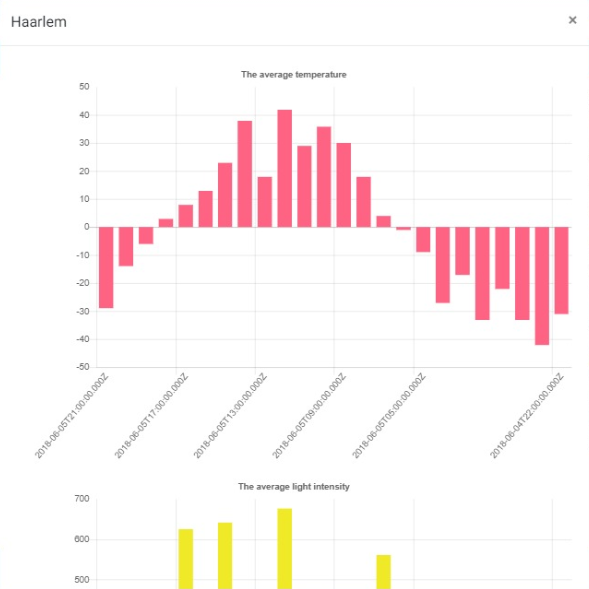
\includegraphics[width=1\textwidth]{sensorhub-popup}
\end{figure}
Note: the full light and gas graphs are not included in this figure.

\newpage
\subsubsection{The heatmap}
If you want to see the temperature measured by the sensor hubs, this is the right option.
The heatmap shows a representation of the temperature, using colors scaling from bright pink (cold) to red (warm). The colors are displayed on the map as a layer over the standard map.
\begin{figure}[h!]
  \caption{Navigation, SensorHubs and Temperature.}
  \centering
  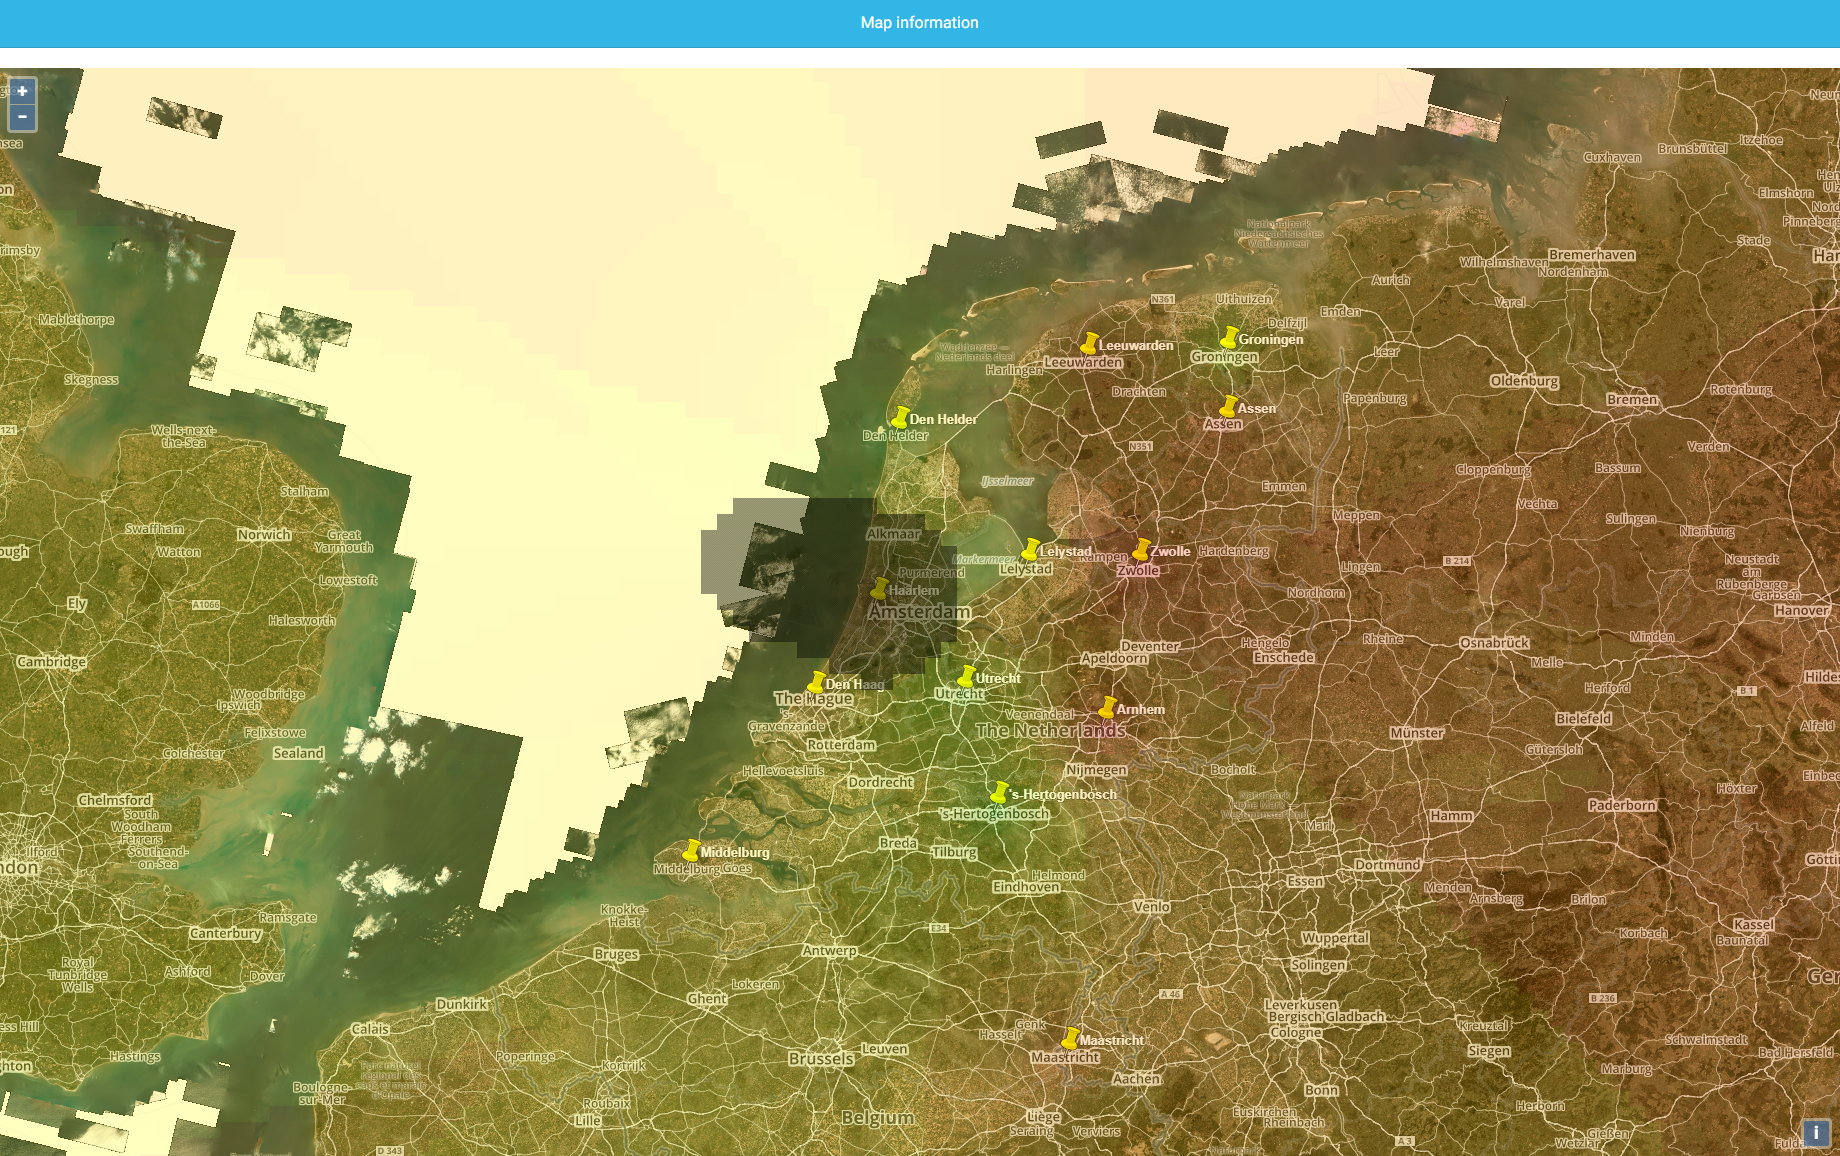
\includegraphics[width=0.9\textwidth]{heatmap}
\end{figure}
\newline

\subsubsection{The gas map} 
The gas map shows the amount of gas that is found on a specific location. The specific location will show the values given of the gas. On the map you will see a number which corresponds to an amount of pollution in the air due to gas.
\begin{figure}[h!]
  \caption{Navigation, SensorHubs and Gasses.}
  \centering
  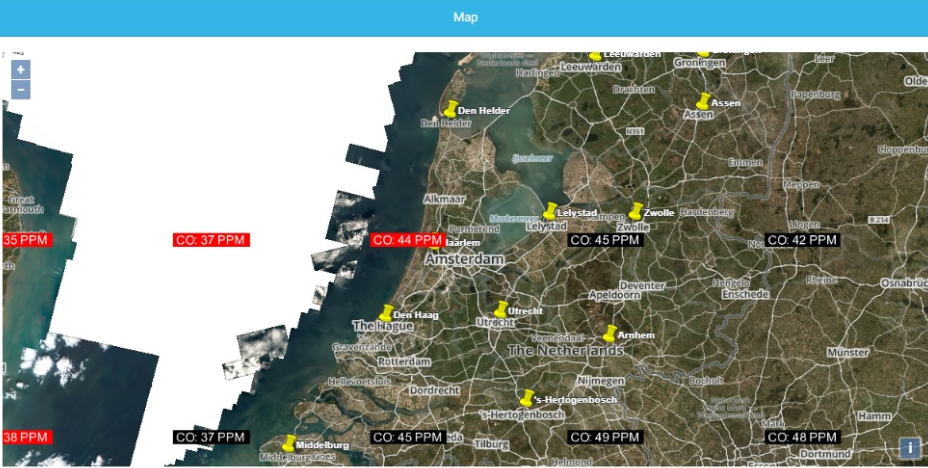
\includegraphics[width=0.9\textwidth]{gasmap}
\end{figure}
\newline

\subsubsection{The light map}
The light map shows the amount of light pollution at a specific location. The light pollution is shown by a lamp icon. The lamp icon has lines above the lamp itself. This is used as our scale. So if the lamp icon has 0 lines it means there isn't any pollution. But if there are 7 lines above the lamp icon it means that there is a lot of pollution going on in the area.
\begin{figure}[h!]
  \caption{Navigation, SensorHubs and Light.}
  \centering
  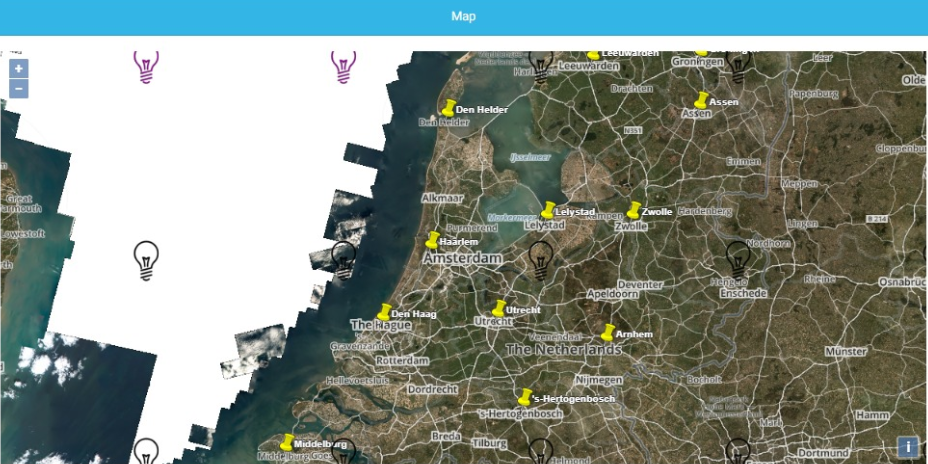
\includegraphics[width=0.9\textwidth]{lightmap}
\end{figure}
\newline

\newpage
\subsection{The admin page}
This page is used to make changes to the system, e.g. user management. Just like the name says, this page is only available for admins. On this page you can change a user's data or that of a sensor hub.
\newline
\newline
This page shows a change logo part and two tables. One table for the users and one for the sensor hubs. With admin rights the user can change the data inside of these tables.
\begin{figure}[h!]
  \caption{Admin page.}
  \centering
  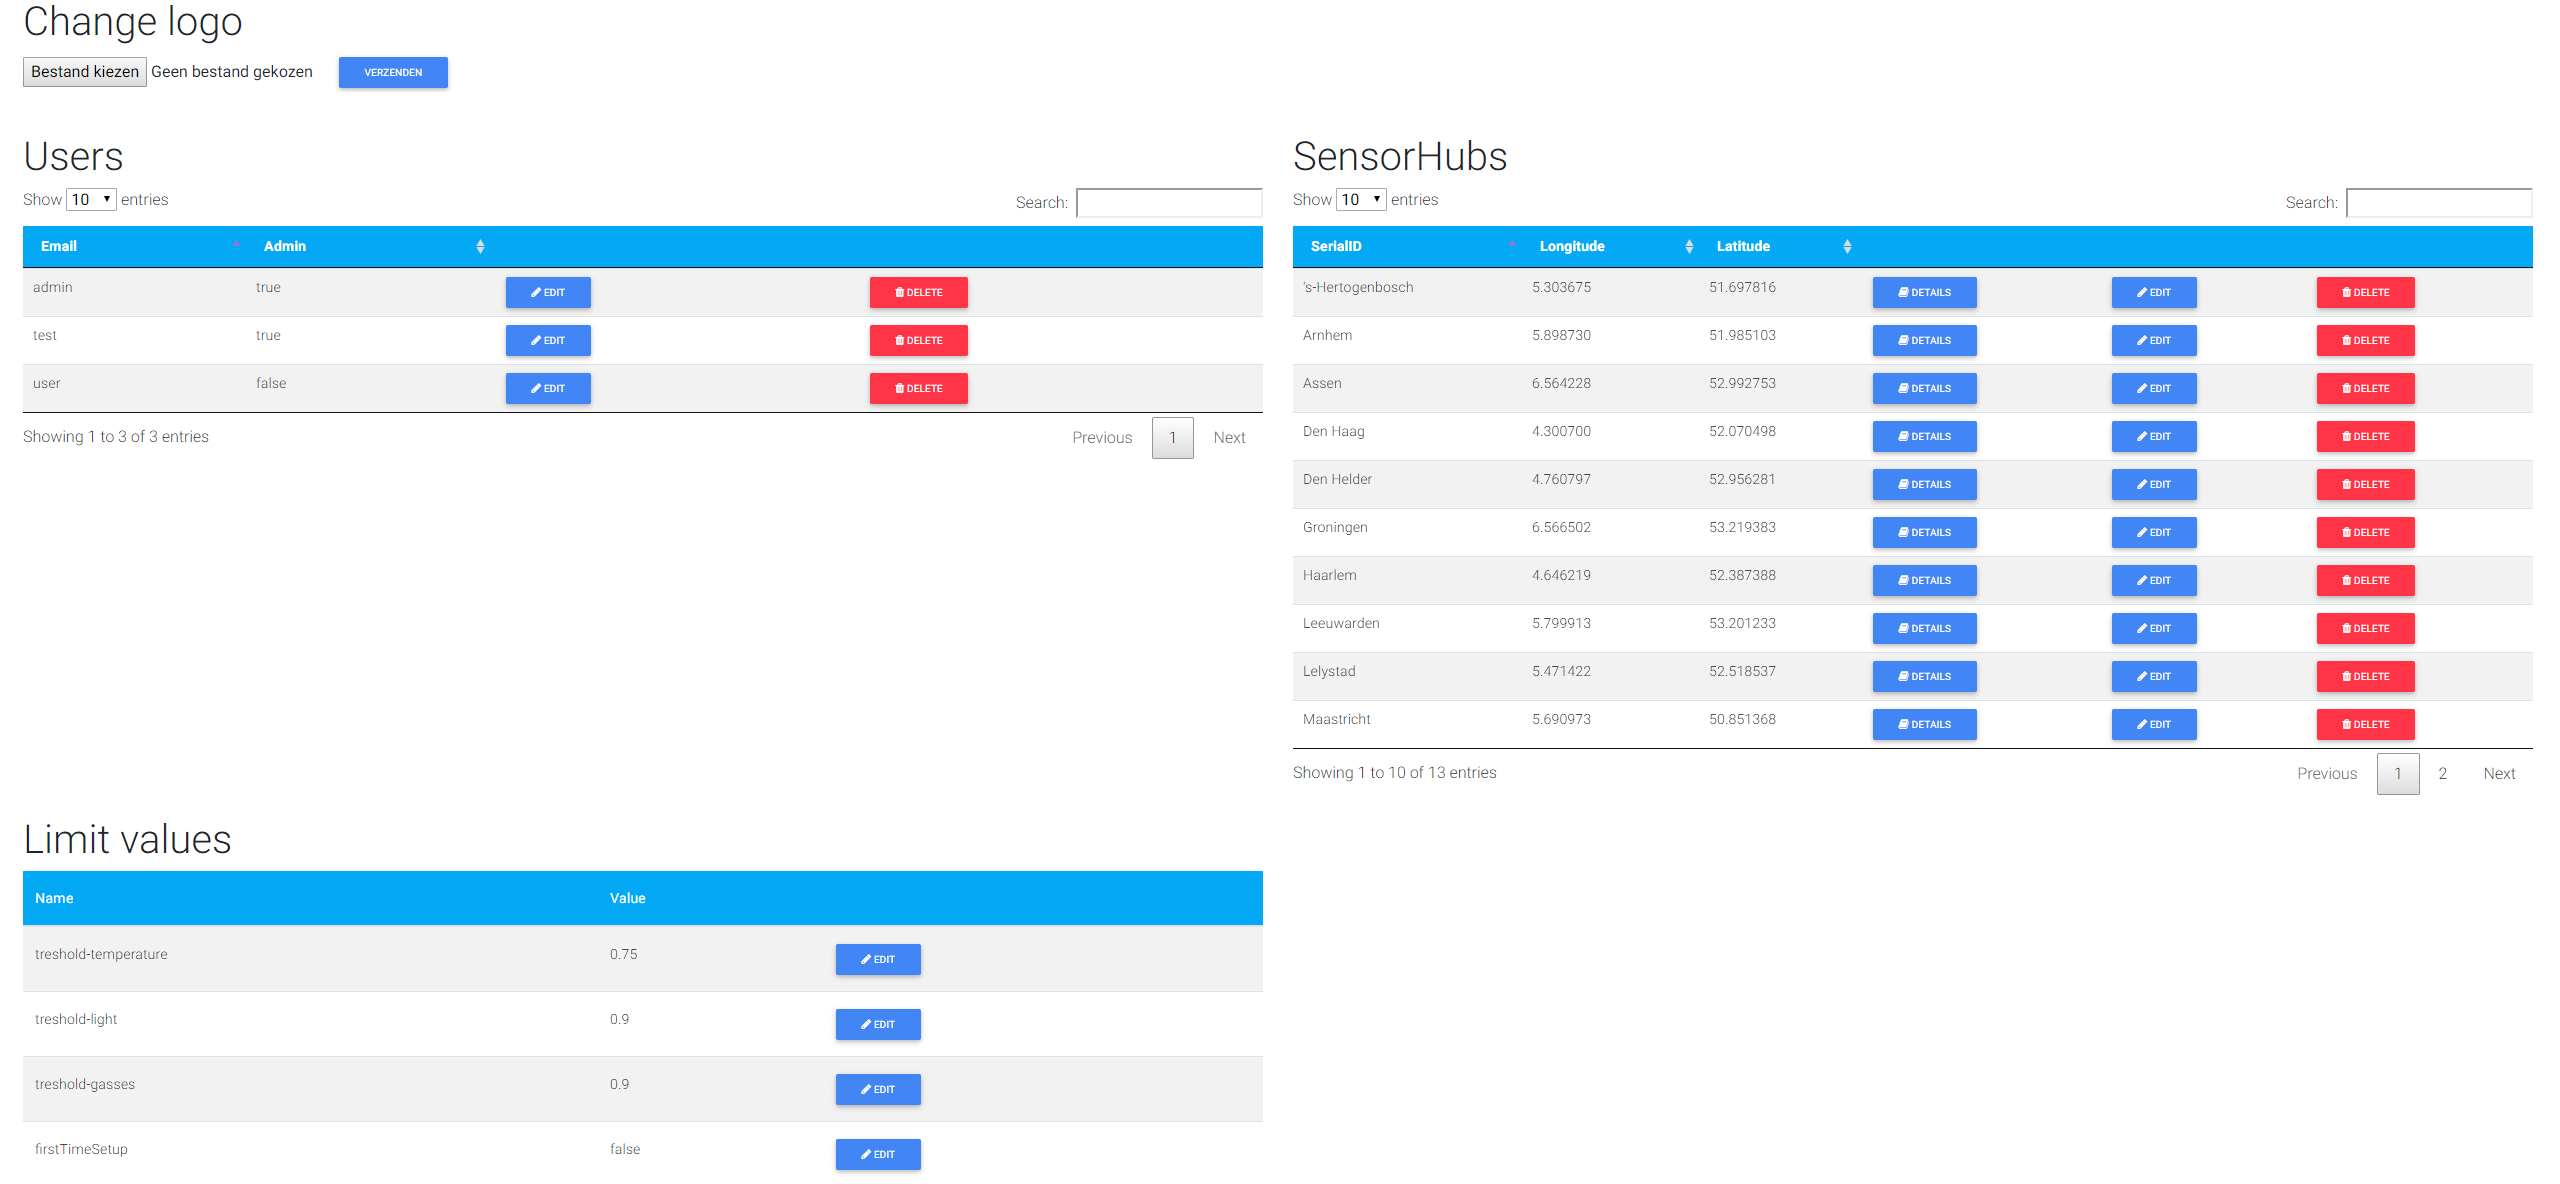
\includegraphics[width=1\textwidth]{admin}
\end{figure}
\newline
\newline
The Users table contains data of all the users. With the add button you can add a user and with the delete button behind a specific user you can delete it. Then there is the edit button. The edit button is used to edit the profile of a specific user.
\newline
\newline
The SensorHubs table simply shows the location of the used sensor hubs with pinpoints. The sensor hub table also contains the same buttons as the users table does.
\newline
\newline
The Limit values table shows the percentage of data around a sensorhub that outputs invalid data is invalid.
\newline
In this case 0.75 at the treshold-temperature means that 75 percent of the data is marked invalid.
\newline
\newline
At the top of the admin page admins are able to change the logo they have the website. There are two buttons, one is named "Bestand kiezen" and the other is called "Upload". With the Bestand kiezen button admins are able to choose a picture from their computer. And with the Upload admins are able to change the logo of the website with the picture they just selected through the Bestand kiezen button.
\newline

\newpage
In the SensorHubs table there is also a button called "Details". When you press on the details button you will be redirected to a different page. On this page you will see all the values in a table of that specific location. On the side of the table you will see a chart. On the chart you will see the same data as in the table but instead of in a table in a chart.
\begin{figure}[h!]
  \caption{The page displaying details of a sensor hub.}
  \centering
  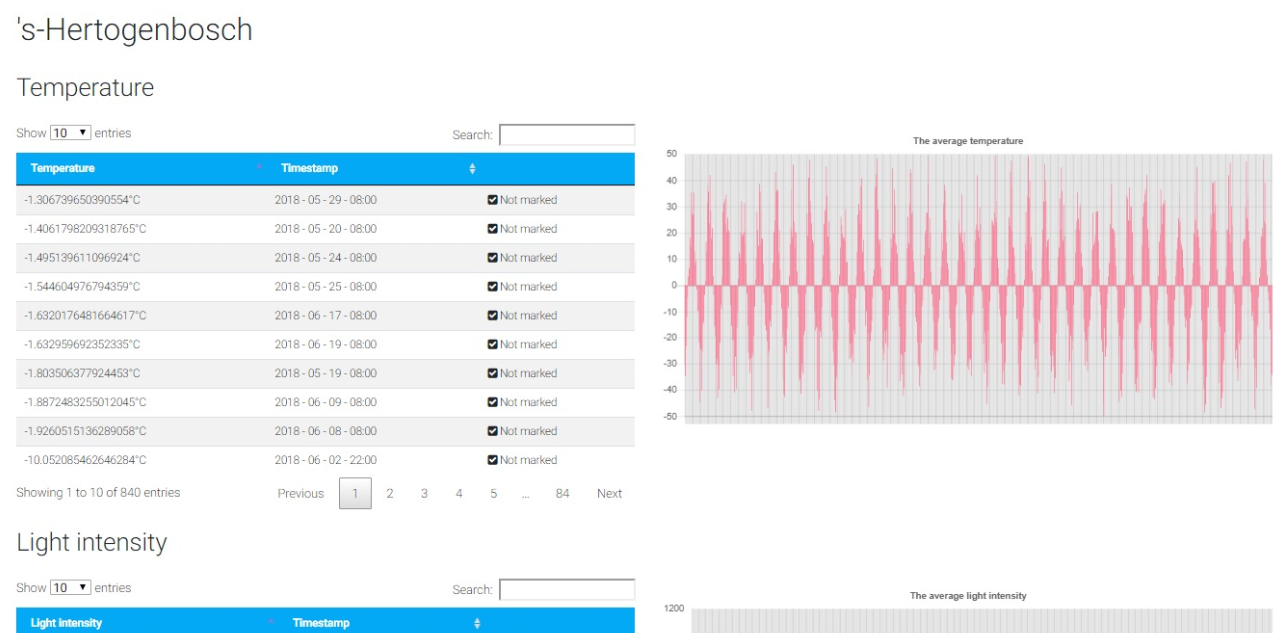
\includegraphics[width=1\textwidth]{admin-details}
\end{figure}

\newpage
\section{Further help}
PLA25 is responsible for making this web application. If any bugs are to be found, please do contact us.
Also contact us if any further help is needed or something is not clear yet.
\newline
\newline
The easiest way to report a bug is through our Github page:
\newline
https://github.com/PLA25/Website/issues

\end{document}
